\documentclass[11pt]{article}
\usepackage[utf8]{inputenc}
\usepackage[labelfont=bf,small]{caption}
\usepackage[compact]{titlesec}
\usepackage{appendix}
\usepackage[noblocks]{authblk}
\usepackage{graphicx,amsmath,booktabs,subcaption,placeins,mathtools,multirow} % All of the classics
\usepackage{tikz}
\usepackage[activate={true,nocompatibility},
    final,
    tracking=true,
    kerning=true,
    spacing=true,
    factor=1100,
    stretch=10,
    shrink=10]{microtype}
    \microtypecontext{spacing=nonfrench}
\usepackage[colorlinks,
    linkcolor=teal,
    citecolor=teal,
    filecolor=teal,
    urlcolor=teal]{hyperref}
\usepackage[margin=1in]{geometry} % 1in margins
\usepackage[version=4]{mhchem}

\DeclareCaptionLabelFormat{withincaption}{#2)}
\captionsetup{subrefformat=withincaption}

% -- Use the Charter fonts as base fonts, fixup math-mode display
\usepackage[charter]{mathdesign}
\usepackage[scaled=.96,osf]{XCharter}
\linespread{1.04}
\usepackage[backend=biber,style=nature,backref=true]{biblatex} %author-year for in-text content
%\hyphenpenalty=750
\usepackage{cleveref}
\crefname{appendix}{supplemental section}{supplemental sections}
%-------------------end standard preamble-------------------------
\newcommand{\units}[2]{\frac{\text{#1}}{\text{#2}}\,}
\newcommand{\unit}[1]{\; \text{#1}\,}

\titlespacing{\section}{0pt}{2ex}{1ex}
\titleformat{\subsection}[display]{\bfseries}{}{0em}{}
\titlespacing{\subsection}{0pt}{0.1em}{0.1em}

\title{DNA supercoiling coordinates transcription via topologically-active networks of genes }
\author{Christopher P. Johnstone}
\author{Kate E. Galloway}
\affil{Department of Chemical Engineering, MIT, 25 Ames St., Cambridge, MA 02139, USA}
\date{ }

\addbibresource{main_library.bib}

\begin{document}
\maketitle

%TODO: add abstract

\section{Introduction}
Cells coordinate complex behaviors through precise spatiotemporal control of gene expression. To rapidly advance gene and cell-based therapies, synthetic biology aims to harness the power of native biology by constructing synthetic gene regulatory networks capable of dynamically prescribing cellular processes, states, and identities.\parencite{chenSyntheticBiologyAdvancing2012,beitzSyntheticGeneCircuits2022,purnickSecondWaveSynthetic2009,elowitzBuildLifeUnderstand2010}
Synthetic networks process diverse inputs into complex logical and temporal responses.\parencite{weinbergLargescaleDesignRobust2017,xieMultiInputRNAiBasedLogic2011,taborSyntheticGeneticEdge2009}
From oscillators to pulse generators, synthetic circuits can  precisely coordinate dynamic patterns of gene expression across populations of cells to control cell fate.\parencite{gardnerConstructionGeneticToggle2000,elowitzSyntheticOscillatoryNetwork2000,strickerFastRobustTunable2008,daninoSynchronizedQuorumGenetic2010,maSyntheticMammalianSignaling2022,parkEngineeringEpigeneticRegulation2019,bashorUsingEngineeredScaffold2008,gallowayDynamicallyReshapingSignaling2013}
However, rational \textit{de novo} design of synthetic circuits remains challenging. Despite extensive biomolecular modeling, integration of single genetic elements into systems often leads to emergent behaviors, requiring iterative design-build-test cycles to achieve the desired performance.\parencite{jonesEndoribonucleasebasedFeedforwardController2020,freiCharacterizationMitigationGene2020,qianResourceCompetitionShapes2017}
Compounding the challenge, transcription exhibits significant extrinsic and intrinsic noise.\parencite{toNoiseCanInduce2010,zopfCellCycleDependenceTranscription2013,desaiDNArepairPathwayCan2021}
In particular, the stochastic nature of transcription makes coordinating expression across multiple genetic elements challenging.\parencite{rodriguezIntrinsicDynamicsHuman2019,rodriguezTranscriptionLivingCells2020,quartonUncouplingGeneExpression2020}
Spatial variation in the nucleus and biochemical dynamics in condensates may contribute to bursting but provide limited parameters for tuning transcriptional noise.\parencite{henningerRNAMediatedFeedbackControl2020,guoPolIIPhosphorylation2019}
Alternatively, mechanical sources of gene regulation offer one potential mechanism by which to understand and harness transcriptional noise to improve the predictable design of gene circuits.\parencite{johnstoneEngineeringCellularSymphonies2021,anconaTranscriptionalBurstsNonequilibrium2019a,kimLongDistanceCooperativeAntagonistic2019,elhoudaiguiBacterialGenomeArchitecture2019a,meyerTorsionMediatedInteractionAdjacent2014}.

The mechanical forces of DNA supercoiling powerfully shape transcriptional variance.\parencite{desaiDNArepairPathwayCan2021,chongMechanismTranscriptionalBursting2014}
Chromatin, the DNA polymer wrapped around nucleosomes and decorated with regulatory proteins, regulates diverse processes from transcription to differentiation. With enhanced resolution in the layers and dynamics of chromatin structure, the manifold functions of chromatin-mediated gene regulation are emerging.\parencite{hsiehResolving3DLandscape2020,krietensteinUltrastructuralDetailsMammalian2020}
In the process of transcription, RNA polymerases induce a leading wave of positive DNA supercoiling\parencite{wuTranscriptionGeneratesPositively1988,liuSupercoilingDNATemplate1987}, reshaping the local structure of chromatin.\parencite{acharNegativeSupercoilGene2020,tevesTranscriptiongeneratedTorsionalStress2014,naughtonTranscriptionFormsRemodels2013,guoHighresolutionGenomewideMapping2021a}
At the kilobase scale, chromatin structure correlates with gene regulation.\parencite{hsiehResolving3DLandscape2020,rowleyEvolutionarilyConservedPrinciples2017}
In yeast and human cells, transcriptionally-induced supercoiling demarks bounds of gene activity.\parencite{acharNegativeSupercoilGene2020,naughtonTranscriptionFormsRemodels2013}
In particular, transcriptional activity dictates the strength of contact domains such as gene-to-gene interactions, indicating a role for transcription in forming and maintaining interactions at the kilobase scale.\parencite{rowleyOrganizationalPrinciples3D2018,rowleyEvolutionarilyConservedPrinciples2017}
Together these data suggest that the process of transcription drives formation of supercoiling-linked, kilobase-scale structures that feedback into transcriptional regulation of gene expression. Biophysical models of gene expression predict that changes in DNA supercoiling in turn change transcriptional activity.\parencite{sevierPropertiesGeneExpression2018}
As supercoiling rapidly diffuses across long distances \parencite{loenhoutDynamicsDNASupercoils2012}, transcriptional activity at one site may impact the overall activity and dynamics of transcription of proximal genes.\parencite{sevierCollectivePolymeraseDynamics2022,tripathiDNASupercoilingmediatedCollective2021}
Understanding how supercoiling induces coupling between neighboring genes provides the opportunity to improve the predictable design of transgenic systems from simple reporters to sophisticated dynamic circuits.

Here we develop a model of transcriptional regulation that integrates DNA supercoiling to examine how the activity of neighboring genes in differing orientations affects expression of both genes. Models of supercoiling-dependent gene expression already exist in the literature \parencite{sevierCollectivePolymeraseDynamics2022,tripathiDNASupercoilingmediatedCollective2021}. However, these models either do not include the influence of supercoiling on polymerase initiation or restrict predictions to relatively inaccessible experimental variables such as RNA polymerase velocity. Additionally, few models examine how supercoiling-dependent behavior interacts with other classic regulatory mechanisms.

We develop a model of supercoiling-dependent polymerase initiation that extends a previously-reported supercoiling-dependent polymerase model.  \parencite{sevierPropertiesGeneExpression2018}  We extend our model with supercoiling-dependent polymerase initiation terms and the ability to simulate arbitrary regulatory interactions, allowing modeling of many classic circuits such as toggle switches relevant both to native and synthetic systems. Using simple two-gene systems, we find that supercoiling-dependent regulation is strongly dependent on both circuit syntax---the relative orientation and position of genetic elements---and the enclosing boundary conditions. In addition to regulating the output of simulated genes, supercoiling-dependent feedback additionally can tune the size and time between successive expression bursts, suggesting an additional mechanism to tune these key variables in synthetic systems. We extend this model to examine a synthetic toggle switch.
We predict how syntax affects DNA supercoiling and the stability of states, examine transition dynamics, and define the critical parameters for designs. Finally, we adapt our model to investigate the explanatory power of DNA supercoiling as a mechanism for coordinating expression between divergently expressed genes in the zebrafish (\textit{Danio rerio}) segmentation network. We find that supercoiling-dependent feedback is capable of tightly regulating proximal clock genes, replicating a key experimental finding and providing a molecular mechanism that supports precise coordination of gene expression during somite formation. \parencite{zinaniPairingSegmentationClock2021}.

\begin{figure}[h]
    \centering
    \includegraphics{figures/modeling_paper/graphical_abstract}
    \caption{Supercoiling-mediated feedback drives emergent regulatory behaviors that depend on the surrounding genetic context.} \label{fig:graphical_abstract}
\end{figure}

\section{Model and methods}
Simulating the behavior of native and synthetic circuits under the influence of transcription-induced feedback requires an model that integrates explicitly-modeled polymerase motion and RNA- and protein-mediated feedback mechanisms.
Our method combines three modeling levels: an ordinary differential equation model that simulates the continuous progression of polymerases loaded onto DNA, a core stochastic model that models supercoiling-dependent polymerase initiation, and a user-specified stochastic layer that allows for modeling other modes of transcriptional regulation such as the promoter-repressive and -activating interactions that are often included in synthetic circuits.

\subsection{Continuous model of supercoiling-dependent transcription}

\begin{figure}[h]
    \centering
    \includegraphics[width=\textwidth]{figures/modeling_paper/variable_supercoiling_explanation}
    \caption{In the limit of fast supercoiling relaxation relative to polymerase motion, the supercoiling density is constant in the region between polymerases. Four key variables define the location of each polymerase: it's linear distance \(z\) along the genome, the length of the nascent mRNA transcript \(x\), the rotation of the polymerase \(\theta\), and the local DNA excess twist \(\phi\). The tradeoff between RNAP rotation and DNA rotation generates supercoiling upstream and downstream, with the drag generated by the nascent mRNA primarily balancing the torque caused by generated supercoils. Using an energy model responsive to local supercoiling, we can derive supercoiling-dependent initiation terms to model differential polymerase loading rates.}
    \label{fig:key_variables_diagram}
\end{figure}
Here, supercoiling is defined as the amount of excess twist \(\phi\) relative to relaxed DNA. Relaxed DNA rotates  one full revolution per \(\approx10\) basepairs (1bp \(\approx 0.34\) nm); thus it's relaxed twist is \(\omega_0 = 1.85\) radians/nm. Supercoiling density can generally be defined as a varying function of genomic location \(\sigma(z)\). However, in a region of constant supercoiling density, we can use the excess DNA twist \(\phi\) at the endpoints \(z_1, z_2\) to conveniently define the supercoiling density as:
\begin{equation}
    \sigma = \frac{\phi(z_1) - \phi(z_2)}{\omega_0 (z_2 - z_1)}
\label{eq:supercoiling_density}
\end{equation}
The relationship in \cref{eq:supercoiling_density} specifies the value of \(\phi\) at any intermediate point \(z_i\) between the two endpoints \(z_1, z_2\). For relaxed DNA where \(\phi=0\), a positive value of \(\phi\) means that the supercoiling density is \emph{positive} in front of the intermediate point and \emph{negative} behind the intermediate point (\cref{fig:key_variables_diagram}). Following on the work of \textcite{sevierPropertiesGeneExpression2018}, we assume that on the length scales of synthetic and native circuits of interest (\(O(\approx10kb)\)), the supercoiling density is constant in all regions between polymerases and other barriers. Because supercoiling diffusion and plectoneme hopping \parencite{loenhoutDynamicsDNASupercoils2012} occur at rates faster (diffusion constant of \(\mathcal{D} \approx O(0.5 \units{kb$^2$}{s})\)) than transcription (\(v_0 \approx 0.05 \units{kb}{s}\)) \parencite{munizRNAPolymeraseII2021}, the supercoiling generated by a polymerase will diffuse outward far more rapidly than polymerases can move. We make a pseudo-steady assumption for inter-RNAP supercoiling---assuming that \cref{eq:supercoiling_density} holds between polymerases---over the relatively small (\(\sim 10\) kb) genomic distances considered in this work in order to simplify the resulting model.

How does transcription both drive the process of supercoiling generation and react to changes in local supercoiling? Under the assumption of supercoiling relaxation, each polymerase is defined by four variables--the one-dimensional genomic location of the polymerase \(z_i\), the length of the nascent RNA \(x_i\), the excess twist at the location of the polymerase \(\phi_i\), and the rotation angle of the polymerase \(\theta_i\) (\cref{fig:key_variables_diagram}). Then, two governing equations define the motion of all polymerases.\parencite{sevierPropertiesGeneExpression2018} The first equates the linear motion of the polymerase with the rotational motion of both the RNAP and the DNA required for the polymerase to track the DNA groove:
\begin{equation}
    \underbrace{\omega_0 \frac{dz_i}{dt}}_{\mathclap{\text{RNAP velocity}}} = \overbrace{\frac{d\theta_i}{dt}}^{\mathclap{\text{RNAP rotation}}} + \underbrace{\frac{d\phi_i}{dt}}_{\mathclap{\text{supercoiling generation}}}
\label{eq:linear_rotational_balance}
\end{equation}
The second equation provides a torque balance between the DNA-mediated torques on the left hand side and the torque caused by drag acting on the nascent RNA:
\begin{equation}
    \underbrace{\tau(\sigma(z_i, \phi_{i-1}, \phi_{i+1}))}_{\mathclap{\text{torque acting on RNAP}}} + \overbrace{\chi \frac{d\phi_i}{dt}}^{\mathclap{\text{supercoiling restoring force}}}= \underbrace{\eta x_i^n \frac{d\theta_i}{dt}}_{\mathclap{\text{nascent RNA drag}}}
\label{eq:torque_balance}
\end{equation}
To develop a final system of ordinary differential equations, we can simplify through introduction of a few definitions. If we define equations for the torque response \(\tau(\sigma)\) as a function of the local supercoiling density and the RNAP velocity as a function of local torque \(\frac{dz}{dt} = v(\tau)\), then \Cref{eq:linear_rotational_balance,eq:torque_balance} can be solved as in \textcite{sevierPropertiesGeneExpression2018}. Here, we use Marko's torque-response model to supercoiling which accounts for the thermodynamic behavior of both non-buckled, twisted DNA and buckled, plectonemic DNA (see \cref{eq:marko_torque,eq:marko_energy} in \cref{sec:appendix:model}) \parencite{markoTorqueDynamicsLinking2007}. The resulting \(\tau(\sigma)\) functions exhibits a phase transition, where the torque response is nearly constant at intermediate values of \(\sigma\) where the DNA is transitioning from a locally-twisted phase to a plectonemic-phase (\cref{fig:supp:torque_diagram}).

For the velocity response of a polymerase experiencing a torque \(\tau_f\) in front and \(\tau_b\) behind, we model polymerase stalling as:
\begin{equation}
    v(\tau_f, \tau_b) = \frac{v_0}{(1 + e^{(|\tau_f| - \tau_s)/\tau_w})(1 + e^{(|\tau_b| - \tau_s)/\tau_w})}
\label{eq:velocity_response}
\end{equation}
where the stall torque \(\tau_s = 12 \unit{pN nm}\) and stall-width \(\tau_w = 3 \unit{pN nm}\) define a sigmoidal stall-response curve.
As shown in \cref{fig:hyperparam_stall_torque,fig:hyperparam_stall_width}, our results are only weakly dependent on the specific choice of \(\tau_s\) and \(\tau_w\).
Importantly, our selected phenomenological term will stall polymerase motion if \emph{either} the torque upstream or downstream exceeds the stall torque \(\tau_s\). Some models choose a stalling equation that only stalls if the difference between the upstream and downstream torque exceeds a stall torque \parencite{tripathiDNASupercoilingmediatedCollective2021}; we chose this form, reasoning that the DNA unwinding and rewinding process opposed, respectively, by upstream and downstream torque could independently stall. When simulated, the difference between these stalling models is small in practice; polymerases at the start or end of the burst encounter both high upstream and downstream torques \emph{and} a high torque difference, whereas polymerases in the middle of a burst experience both low adjacent torques and a low torque difference.

Taking the above equations together, we can simulate the coupled motion of an arbitrary number of polymerases as a single coupled ODE system. We further examine different experimental systems by implementing different boundary conditions that allowed us to simulate both plasmid systems and genomically-integrated systems (see \cref{sec:appendix:bcs}).

\subsection{Modeling supercoiling-dependent initiation}
With the ability to simulate arbitrary numbers of polymerases, we need a way to model the addition of polymerases to simulated genes. A simple strategy is to assume a supercoiling-independent initiation rate and use a stochastic simulation method to randomly add polymerases to transcriptional start sites at a certain fixed rate. However, this simple model assumes that polymerases can bind equally well to initiation sites independent of local supercoiling, missing supercoiling-dependent dynamics. In order to include supercoiling in a polymerase initiation model, we relate the basal expression rate to a corresponding base energy term. We can then additively introduce extra energy costs for polymerase binding under different local supercoiling conditions. Under the approximation that the direct energetic cost of locally melting the DNA to fit in the RNAP groove dwarfs the relative change in unwinding energy caused by supercoiling, the majority of the energetic cost comes from inserting supercoiling ahead and behind the inserted polymerase. Under this assumption, the first-order supercoiling energetic correction can be written as:
\begin{equation}
    E_\text{sc} = 1.2  \cdot 2\pi \cdot \tau(\sigma)
\label{eq:first_order_sc_initation}
\end{equation}
 Is this a good approximation? We can estimate the energetic cost of local melting, and find that neglecting local melting leads to a minor change in the resulting energy as seen in \cref{fig:supp:energy_with_melting}. A full derivation of these results is given in \cref{sec:sc_initation}.

While this first-order energetic term introduces much-needed behavior to the modeled system---where locally high positive supercoiling decreases the RNAP initiation rate and locally negative supercoiling increases the RNAP initiation rate---at extreme values of \(\sigma\), this energetic term gives aphysical predictions. In particular, under highly negative supercoiling densities, the energetics of polymerase loading becomes increasingly favorable, with loading sometimes occurring more than two orders of magnitude faster when compared to relaxed DNA. To correct for behavior, we add a second-order (quadratic) term of the form that constrains polymerase loading at highly positive or negative local supercoiling:
\begin{equation}
    E_\text{sc} = 1.2  \cdot 2\pi \cdot \tau(\sigma) + \alpha \cdot \tau_0 \cdot \sigma^2
\label{eq:second_order_sc_initation}
\end{equation}
for \(\tau_0\), the relevant scale factor in the \(\tau(\sigma)\) equation \parencite{markoTorqueDynamicsLinking2007} and \(\alpha\) a positive tunable parameter. As the \(\tau(\sigma)\) equation is linear in \(\sigma\) outside of the phase-transition region, this added \(\sigma^2\) term can be contextualized as an additional term in the Taylor expansion of the physically-realistic \(E_\text{sc}(\sigma)\) equation.

For these three models of supercoiling-dependent initiation,we found that the supercoiling-independent initiation model predicted only small fold changes in reporter output (\cref{fig:supp:initation_order_comparison}). Comparing the first- and second-order models, we found that a critical value of \(\alpha\) existed, \(\alpha \approx 0.2\), above which the second-order model demonstrated emergent non-monotonic behavior (\cref{fig:top:alpha_sweep}). At low values of \(\alpha\), the second-order model behaves similarly to the first-order model, so we used \(\alpha = 0.025\) for this work. Increasing \(\alpha\) beyond this chosen value appears to scale down reporter output without qualitatively modifying behavior (\cref{fig:top:alpha_sweep}).


When simulating the ODE model, the rate of stochastic polymerase initiation, \(r_\text{initiation}\), then varies continuously based on the local supercoiling density \(\sigma\) at the transcription start site as:
\begin{equation}
    r_\text{initiation} = r_\text{base rate} \cdot e^{- E_\text{sc} / (k_B T)}
\label{eq:intermediate_init_rate}
\end{equation}


\subsection{Modeling additional stochastic, discrete reactions}
Many of the native and synthetic systems of interest include mechanisms of gene regulation that rely on other regulatory species. In order to analyze these types of systems using our supercoiling model, we extended our model to simultaneously simulate arbitrary discrete stochastic equations---such as those commonly used in the literature to model protein production, degradation, dimerization, and more. This addition allowed us to model discrete events otherwise not accounted for in the continuous model. Importantly, we simulated the activity of topoisomerases in this way, modeling topoisomerase activity as a stochastic event that removed accumulated supercoiling within intergenic regions.

In addition, we allowed the base initiation rate of genes to vary as an arbitrary function of all species concentrations in the model, such that \cref{eq:intermediate_init_rate} becomes:
\begin{equation}
    r_\text{initiation} = r(\text{modelled species}) \cdot e^{- E_\text{sc} / (k_B T)}
\label{eq:final_init_rate}
\end{equation}
By combining discrete reactions with the ability to dynamically change polymerase initiation rates, we are able to simulate a wide range of phenomena.
For example, a cooperative repressive interaction between some repressor protein \(R\) and a promoter could be modeled using a repressive Hill function:
\[
    r_\text{initiation}(R) = \frac{e^{-E_\text{sc} / (k_B T)}}{1 + \left(\frac{R}{K}\right)^n}
\]
More generally, we can use stochastic formulations of other regulatory mechanisms and test how these mechanisms behave in concert with supercoiling-mediated feedback.

\section{Results}

\subsection{DNA supercoiling dynamics confer rapid, tunable coupling between adjacent genes}
In order to characterize the behavior of supercoiling-mediated feedback, we simulated a series of simple two-gene systems. In addition to being experimentally accessible, two-gene systems allow us to test and understand the core design considerations---syntax, relevant boundary conditions, and experimentally tunable model parameters---while still retaining interpretability. Our two-gene systems consist of a reporter gene that is constitutively active and an adjacent, inducible gene placed in either a tandem orientation with the reporter upstream, tandem orientation with the reporter downstream, convergent orientation, or divergent orientation (\cref{fig:base_orientations}).


Transcriptional noise and the ability of circuits to respond or suppress noise is integral to the functioning of native and synthetic systems. For an ensemble of cells, the population variance can be decomposed into an \emph{extrinsic} noise component that describes how the all genes co-vary within a cell and an \emph{intrinsic} noise component that describes the inter-gene variance within a cell. To investigate how syntax impacts noise, we examined an ensemble of linear two-gene systems, where the base rate of both the reporter and the inducible gene were set to be equal (e.g. one-fold induction) (\cref{fig:output_distribution_by_orientation}). We found that while the tandem syntaxes showed approximately equal intrinsic and extrinsic noise, the convergent and divergent populations showed shifts in the variance distribution.
The divergent syntax showed an increase in extrinsic noise concomitant with a decrease in intrinsic noise.
In contrast, the convergent population showed an increase in intrinsic noise and a decrease in extrinsic noise. Here, fluctuations in the number of polymerases on one of the genes drives the accumulation of positive supercoiling at the other gene's promoter, reducing its output. This self-reinforcing interaction tends to enhance inter-gene variance. Clearly, circuit syntax can be a powerful tool in tuning circuit noise behavior.


Observing the substantial role that supercoiling accumulation plays in these systems' behavior, we examined how boundary conditions and inter-gene spacing tune behavior. Experimental systems provide both  circular and linear boundary conditions including  plasmids and genomically-integrated cassettes constructs, respectively. Because circular boundary conditions represent the common experimental system of transient transfection of plasmids, we extended our simulation to circular boundary conditions using the same three circuit syntaxes and the second-order polymerase initiation model (\cref{fig:reporter_output_by_bc}). At low induction of the adjacent gene, circular boundaries conditions generate lower reporter output across syntaxes compared to linear boundary conditions. When compared to the linear boundary condition simulations,  circular boundary conditions support similar behavior in the convergent and divergent syntaxes, showing a monotonic increase in reporter output as a function of adjacent induction. In fact, for \(\alpha < 0.02\), the convergent and divergent reporter output curves are effectively identical (\cref{fig:supp_alpha_sweep_circular}).
Moving forward, we used the linear set of boundary conditions to analyze system behaviors as we observe the richest set of behaviors under these boundary conditions.

As the supercoiling \emph{density} is the key variable in determining both polymerase stalling and supercoiling-dependent initiation, changing the intergene spacing directly changes the amount of generated supercoils are required to reach some fixed supercoiling density(\cref{fig:intergene_spacing_cartoon}). For the circuits in \cref{fig:reporter_output_by_init_type,fig:reporter_output_by_bc,fig:output_distribution_by_orientation}, the intergene spacing was set at 2kb. To understand the spacing-driven deviations in reporter behavior, we simulated our linear two-gene circuits with different intergene spacings from 500bp to 10kb and plotted the output of each circuit, relative to the 10kb case. As seen in \cref{fig:reporter_output_by_spacing_fold_induction}, changes in inter-gene spacing mildly influenced expression in the tandem and divergent syntaxes. However, across most induction levels of the adjacent gene, the convergent syntax showed a strong \emph{reduction} in reporter output. Thus, the convergent syntax appears particularly sensitive to accumulation of positive supercoiling in the intergenic region,which may enhance polymerase stalling.

\begin{figure}[h]
    \centering
    {\includegraphics[width=\textwidth]{figures/modeling_paper/fig_base_model.pdf}
    \phantomsubcaption\label{fig:base_orientations}
    \phantomsubcaption\label{fig:linear_bc_distributions}
    \phantomsubcaption\label{fig:circular_bc_distributions}
    \phantomsubcaption\label{fig:linear_fold_induction}
    \phantomsubcaption\label{fig:circular_fold_induction}
    \phantomsubcaption\label{fig:intergene_spacing_cartoon}
    \phantomsubcaption\label{fig:reporter_output_by_spacing_fold_induction}}
    \phantomsubcaption\label{fig:base_model_sc_density}
\end{figure}
\begin{figure}
    \ContinuedFloat
    \caption{Supercoiling-dependent polymerase motion and polymerase initiation predict context-dependent circuit behavior.
        \subref{fig:base_orientations} Two genes were placed into four different orientations as a testbed for understanding context-dependence driven by supercoiling. All four orientations include a reporter gene (gray) and an inducible gene (colored).
        \subref{fig:linear_bc_distributions} For equal basal expression rates between the reporter and inducible gene for the systems with linear boundary conditions, gene orientation dramatically affects the expression distributions. The two tandem orientations behave nearly symmetrically, whereas the convergent and divergent orientations show enhanced intrinsic and extrinsic noise, respectively.
        \subref{fig:circular_bc_distributions} With circular boundary conditions and equal basal expression rates, extrinsic noise dominates the expression distributions for all orientations. The convergent and divergent orientations show especially strong extrinsic noise.
        \subref{fig:linear_fold_induction} Reporter output for the linear boundary condition orientations show non-monotonic behavior as a function of adjacent induction. The upstream tandem and divergent orientations
        \subref{fig:circular_fold_induction} For circular boundary conditions, reporter output tends to increase as a function of fold induction.
        \subref{fig:intergene_spacing_cartoon} Modifying the inter-gene spacing tunes circuit behavior by changing the amount of accumulated supercoils needed to affect polymerase stalling and supercoiling-dependent initiation.
        \subref{fig:reporter_output_by_spacing_fold_induction} Deviations in reporter output relative to the maximum intergene-spacing is shown as a function of intergene-spacing. The convergent orientation is most strongly affected by inter-gene spacing.
        \subref{fig:base_model_sc_density} The supercoiling density across the linear constructs are shown as a function of induction of the inducible gene. At 0-fold induction, positive and negative supercoiling accumulates upstream and downstream of the reporter gene, respectively. Context-dependent behavior is demonstrated when the adjacent gene is activated.
    } \label{fig:top:orientation_bc_behavior}
\end{figure}

\FloatBarrier
\subsection{Supercoiling drives correlated ensemble behavior by tuning burst frequency and single cell expression patterns.}

To understand the mechanisms that support syntax-specific expression profiles \cref{fig:top:orientation_bc_behavior}, we examined the ensemble supercoiling density and burst behaviors of our two-gene systems. Putatively, differences in supercoiling across the two-gene systems give rise to differences in RNAP initiation and thus impact gene expression. To observe supercoiling across the two-gene systems, we averaged the supercoiling density across the simulated ensemble. To examine how induction of the adjacent gene changes supercoiling density, we compared the profiles for when the adjacent gene is uninduced (zero-fold induction) and induced (one-fold induction). As expected, the uninduced cases uniformly showed that positive supercoiling accumulates upstream of the constitutively-active reporter gene while negative supercoiling accumulates downstream(\cref{fig:base_model_sc_density},\cref{fig:supp:sc_density_induction}). Upon induction, supercoiling accumulates within the intergenic regions in a syntax-specific manner.

Experimentally, it is observed that transcription occurs in bursts of activity, and native and synthetic mechanisms can modify burst dynamics \parencite{desaiDNArepairPathwayCan2021,chongMechanismTranscriptionalBursting2014,poppAlteringTranscriptionFactor2021}.
In our model, stochastic polymerase addition leads to transcriptional bursting. In order to understand how circuit syntax contributes to supercoiling-mediated burst dynamics, we examined the distribution of both \emph{burst size}, which we define as the number of polymerases added during a burst, and \emph{inter-burst time}, the amount of time separating two consecutive bursts for the reporter gene (\cref{fig:burst_dynamics_cartoon}). Here, we defined bursts using a burst threshold of 30 seconds, such that a burst was considered to end if 30 seconds passed without a polymerase being added. We observed only small variations in the qualitative differences in burst size and inter-burst time distributions for other choices of the burst threshold (\cref{fig:top:burst_threshold}).

Across the available syntaxes, we found that the burst size distributions in the adjacent-uninduced case (gray lines) were remarkably similar, but displayed syntax-dependent behavior upon induction of the adjacent gene (\cref{fig:base_model_burst_size}). The tandem-reporter-downstream and convergent syntaxes showed a strong decrease in burst size that we attribute to reduced polymerase loading as a result of accumulated positive supercoiling. In contrast, induction of the adjacent gene increased the burst size of the reporter gene, putatively due to enhanced polymerase loading facilitated by accumulated negative supercoiling. Examining the inter-burst time distributions, the tandem-reporter-upstream and divergent syntaxes show a shift to smaller inter-burst times (e.g. shorter promoter ``downtime''; more frequent bursting) (\cref{fig:base_model_interburst_time}). Interestingly, the inter-burst time in the tandem-reporter-downstream and convergent syntaxes appears unaffected by adjacent induction. Together these observations suggest that syntax provides a parameter for orthogonally tuning burst size and burst frequency.


To examine the effects of supercoiling-driven feedback beyond the mean ensemble behavior, we investigated the dynamic behavior of individual simulations. To assess how the induction of transcription of the neighboring gene impacts dynamics between genes with different syntax under linear boundary conditions,
we initialized our two-gene circuits with only the reporter gene being active. After a settling period, we induced transcription of the adjacent gene.
We verified that systems initialized with one active gene recapitulate the mean ensemble behavior at steady state (\cref{fig:supp:fig_examples_ensemble_behavior}), indicating that the systems converge to the same averages independent of initial condition; in other words, our system appears to be ergodic. Thus, we can observe relevant dynamics when initializing the system with only the reporter gene active.

We observe that dynamics vary extensively by syntax (\cref{fig:orientation_examples}). When comparing the two tandem orientations, we observe strong biasing of expression towards the upstream gene with stochastic bursts of expression from the downstream gene. While this upstream dominance does not completely disable the downstream gene, activation of the upstream gene reduces the average expression of the downstream reporter. In the convergent syntax, we observe anticorrelated dynamics, with ``either-or'' promoter activity. In contrast, the divergent syntax supports high levels of expression from both genes. The reporter gene remains active after induction of the adjacent gene. When we plot the ensemble-averaged supercoiling density before and after adjacent induction in \cref{fig:sc_density_turn_on}, we observe similar behavior to \cref{fig:base_model_sc_density}, where positive and negative supercoiling accumulate in the intergenic region of the convergent and divergent syntaxes, respectively. Accumulated positive supercoiling would support the either-or convergent behavior by inhibiting polymerase initiation at the adjacent gene. Due to stochastic fluctuations, the active genes often swap. In contrast, in the divergent syntax, the accumulated negative supercoiling enhances polymerase loading of both genes, leading to high output expression.

To further our understanding of the emergent supercoiling-dependent correlative behavior, we computed the cross-correlation between the gene outputs following induction. The cross-correlation of two signals is itself a function of a time offset; the cross-correlation at some offset time \(\tau\) can be thought of as the Pearson correlation coefficient between the two signals where one has been shifted by \(\tau\) (\cref{fig:cross_correlation_cartoon}). In particular, periodic but out-of-phase signals have appear as strong negative and positive peaks on a cross-correlation plot, with the time offset of peaks corresponding to the phase offset between the signals.

The four syntaxes show starkly different cross-correlation behavior (\cref{fig:orientation_cross_correlation}). The convergent syntax system displays the most striking correlative behavior \cref{fig:orientation_cross_correlation}. The convergent system shows a very large anti-correlation at zero time offset and positive correlation peaks at offsets around \(\pm 2\) hours. This combination suggests a periodic but out-of-phase behavior between the two genes with a period of around one hour, as seen in the example simulation in \cref{fig:orientation_examples}. At all plotted levels of adjacent induction, the divergent syntax shows a strong positive peak at zero time offset, showing strong, aperiodic correlated behavior.
In addition, strong correlative behavior can also be seen in the tandem case where the upstream gene is induced. Weak induction of the upstream gene induces a strong positive correlation, suggesting that weak upstream induction can induce correlated gene output. However, at higher induction levels, the activity of the upstream gene dominates, effectively repressing the downstream gene as observed in \cref{fig:orientation_examples}.

We then examined how adjacent induction affected the time-independent reporter output distributions. Plotting the normalized reporter output distributions both before (dotted) and after (solid) adjacent induction, we find that the behavior exemplified in \cref{fig:orientation_examples} generalizes to the entire ensemble (\cref{fig:output_distribution_by_orientation_dynamics}). The tandem-reporter-downstream and convergent cases show a reduction in reporter output, the tandem-reporter-upstream shows a small increase in reporter output, and the divergent output stays constant. We also noted that the width of the distributions noticeably changed before and after induction.

As noise impacts the properties of native and synthetic gene networks, we quantified the width of the these distributions by plotting the standard deviation of the reporter output as function of time (\cref{fig:noise_by_orientation}). Prior to induction of the second gene, all four systems display similar standard deviations. Syntax differences emerge upon induction of the second gene. We found that syntax strongly modulates the noise behavior of the reporter. In particular, the downstream reporter in the tandem syntax and the reporter in the convergent syntax show a strong \emph{increase} in noise levels while the upstream reporter in the tandem syntax and the reporter in the divergent syntax show a small \emph{decrease} in noise levels. These changes in noise can be understood in light of the change in burst dynamics presented in \cref{fig:base_model_burst_size,fig:base_model_interburst_time}.
The reduction of noise and mean expression value in the tandem-reporter-downstream and convergent cases occurs concomitant with a \emph{decrease} in the burst size (\cref{fig:base_model_burst_size}). This is expected; if each burst is on average smaller, fluctuations in burst size will have a more dramatic effect on each individual simulation. The decrease of noise in the tandem-downstream and divergent syntaxes is matched by a decrease in the inter-burst time (\cref{fig:base_model_interburst_time}). Because bursts happen more frequently, the ensemble reporter output is more stable as we approach the always-on limit.
Taken as a whole, syntax provides a powerful design parameter for inducing and tuning time-dependent behaviors between genes and shaping output gene distributions.

\begin{figure}[htbp]
    \centering
    {\includegraphics{figures/modeling_paper/fig_sc_behavior}
    \phantomsubcaption\label{fig:sc_examples_convergent_divergent}
    \phantomsubcaption\label{fig:sc_density_convergent_divergent}
    \phantomsubcaption\label{fig:burst_dynamics_convergent_divergent}
    \phantomsubcaption\label{fig:sc_examples_tandem}
    \phantomsubcaption\label{fig:sc_density_tandem}
    \phantomsubcaption\label{fig:burst_dynamics_tandem}
    \phantomsubcaption\label{fig:cross_correlation_cartoon}
    \phantomsubcaption\label{fig:orientation_cross_correlation}
    \phantomsubcaption\label{fig:output_distribution_by_orientation_dynamics}
    \phantomsubcaption\label{fig:noise_by_orientation}
    }
\end{figure}
\begin{figure}[htbp]
    \ContinuedFloat
    \caption{Our supercoiling model predicts emergent coupling and noise behavior at a single-cell level.
        \subref{fig:sc_examples_convergent_divergent} mRNA counts from example simulation runs for the convergent and divergent syntaxes are shown. The adjacent gene (gray) is enabled after ten thousand seconds (2.8 hours).%TODO: add labels above each plot "Convergent", "Divergent"
        \subref{fig:sc_density_convergent_divergent} The mean supercoiling density across the convergent and divergent ensembles is shown before and after adjacent gene activation.
        \subref{fig:burst_dynamics_convergent_divergent} The ensemble distribution of burst size (number of polymerases within a burst) and inter-burst time (gap between successive bursts) is compared for the convergent and divergent syntaxes.
        \subref{fig:sc_examples_tandem} mRNA counts from example runs are shown for the upstream and downstream tandem syntaxes.
        \subref{fig:sc_density_tandem} The mean supercoiling density across the tandem ensembles shows strong positive and negative supercoiling accumulation post-induction. %TODO: move the t<2.8 hr and add more sigma labels.
        \subref{fig:burst_dynamics_tandem} The ensemble distribution of burst size and inter-burst time is compared for the two tandem syntaxes.
        \subref{fig:cross_correlation_cartoon} The cross-correlation of two signals \(f(t), g(t)\) at a time offset \(\tau\) can be calculated by `sliding' one mean-centered signal relative to the other mean-centered and integrating the product of the resulting signals.
        \subref{fig:orientation_cross_correlation} The cross-correlation between the two genes is shown for the equal-induction case across the four syntaxes. The convergent and divergent syntaxes showed the strongest cross-correlation, with the convergent case showing periodic behavior and the divergent showing strong correlated expression.
        \subref{fig:output_distribution_by_orientation_dynamics} Distributions of the reporter output before \textit{(dotted)} and after \textit{(solid)} induction of the adjacent gene shows changes in both the mean and standard deviation due to adjacent expression.
        \subref{fig:noise_by_orientation} Ensemble noise behavior for the four simulated syntaxes is shown by plotting the standard deviation of the reporter gene as a function of time.
    }
    \label{fig:top:single_cell_noise_correlation}
\end{figure}

\FloatBarrier
\subsection{Optimizing toggle switch performance and stability through circuit syntax}
From oscillators to pulse generators, synthetic circuits can  precisely coordinate dynamic patterns of gene expression across populations of cells to control cell fate. Yet, \textit{de novo}
design of synthetic circuits remains challenging. Emergent dynamics, mediated through DNA supercoiling, may support or impede the performance of dynamic circuits. The behavior of a simple toggle under the additional influence of supercoiling-mediated feedback is an ideal testbed to understand how syntax influences circuit performance.
Toggle switches and higher-order synthetic circuits built from toggle switches have been well-characterized both theoretically \parencite{gardnerConstructionGeneticToggle2000} and experimentally \parencite{yeungBiophysicalConstraintsArising2017,zhuSyntheticMultistabilityMammalian2021}.
A straightforward toggle switch can be constructed with two genes that mutually repress each other (\cref{fig:toggle_cartoon}); such a switch exhibits two stable basins. If modeled with a continuous, noise-free equations, a toggle switch will remain within one of the basins based on the initial conditions \parencite{gardnerConstructionGeneticToggle2000}. If  we treat the mRNA concentration discretely with a stochastic simulation, the system escapes the stable basin with a certain probability, depending on the size of fluctuations relative to the steady-state values. How does supercoiling-mediated feedback impact this probability of escape? How might supercoiling-mediated feedback interact with mutual transcriptional repression and alter toggle switch behavior?

To answer these questions, we simulate the behavior of a two-gene toggle switch with our model for various circuit syntaxes. To establish the conventional dual repressor system used for toggle switches, we abstracted the regulatory interaction of the repressors using a Hill function to define the base promoter initiation rates:
\begin{equation}
    r_A = r_0 \frac{K_A}{K_A + [B]^n} \qquad r_B = r_0 \frac{K_B}{K_B + [A]^n}
\end{equation}
for \(r_0 = 1/160 \,\text{s}^{-1}\). Here, we do not explicitly model protein production. Rather, transcriptional repression directly depends on the mRNA counts of represessors, as this allows us to understand the behavior of the system without introducing additional rate constants. The half-max value \(K\), the mRNA count at which the promoter activity is half that of \(r_0\), is chosen here to approximately match the mean steady-state value of either stable state. With this convention, we ensure that the toggle switch operates in the regime of maximum sensitivity. In order to compare the behavior of the toggle switches composed with different syntaxes, we initialized each toggle switch within one of the stable basins and induced the second gene after ten thousand seconds (\(\sim3\) hours). The system then evolves under simultaneous mutual inhibition from expression of the repressors as well as from supercoiling-dependent feedback.

Circuit syntax specifies unique toggle switch dynamics that can be understood by visualizing the distribution of mRNA counts over time (\cref{fig:toggle_basin_stability_over_time}). Initially, nearly all of the simulations in the ensemble lie along the axis corresponding to the gene initially expressed. As time progresses, each ensemble approaches and fluctuates around an equilibrium.
The vast majority of the simulations in the tandem syntax remain in or transition to the upstream-active state. In contrast, the convergent syntax approaches an equilibrium where approximately half of the population distributes into each state. With divergent syntax, the toggle distributions converge toward monostablity with low differential expression of either gene.

In the convergent syntax, activation of either gene causes positive supercoiling to accumulate in the intergenic region, enhancing negative regulation. Because of this, we see that the population continues to show bimodal behavior. However, while positive supercoiling enhances the stability of either state while the target gene is active, supercoiling-mediated feedback can quickly change if the alternate gene stochastically activates. The separation of timescales between the supercoiling-mediated feedback and the slower mRNA-mediated regulation still allows the convergently-oriented state to stochastically flip states.

In contarst, the divergent case shows a nearly unimodal population in \cref{fig:toggle_basin_stability_over_time}, due to the correlated expression caused by accumulated negative supercoiling in the intergenic region.
Finally, the tandem-syntax toggle switch shows asymmetric stability. As expected from the tandem dynamics observed in \cref{fig:top:single_cell_noise_correlation}, the state with an active upstream gene remains substantially more stable than the state with an active downstream gene. In the case of the toggle, the tandem syntax provides the extremes of stability, with the asymmetry arising from the sign of the supercoiling that accumulates at the promoter. When the upstream gene is active in tandem, positive supercoiling accumulates at the downstream promoter, reducing RNAP binding and reinforcing repressor-mediated negative regulation. However, when the downstream gene is active in tandem, negative supercoiling accumulates at the upstream promoter, increasing the rate of RNAP binding, weakening the negative regulation, and resulting in slow state switching.

To quantify these distribution results, we computed the \emph{stable fraction} of the ensemble, defined as the fraction of simulations that have never left the initial starting basin at a certain simulation time.
The stable fraction monotonically decreases toward zero with time, as simulations that cross into the other stable basin are no longer counted as stable even if they return to the original basin.
We observe substantial syntax differences in the dynamics of the stable fraction of the ensemble (\cref{fig:toggle_stable_frac_n_2.0}). While the tandem orientations represent the extremes of stability, the convergent and divergent syntaxes exhibit intermediate stabilities, putatively due to the influence of the accumulated positive and negative supercoiling at the promoter regions deferentially stabilizing or destabilizing mutual inhibition.

Accumulated supercoils also tunes toggle switch behavior by modifying expression burst dynamics. In particular, we observe that the divergent syntax displays \emph{reduced} burst size when compared to the other syntaxes (\cref{fig:toggle_burst_size}). This observation may suggest that the behavior of the divergent toggle switch is governed by a conflicting interaction at the promoter level between supercoiling-mediated feedback and mutual inhibition.
Overall, these trends suggest that toggle switch behavior emerges through correlated (or anti-correlated) transcription rather than through differences in burst size and inter-burst time, pointing to potentially orthogonal modes of tuning expression of toggle genes.

While circuit syntax provides a powerful tool for tuning toggle switch behavior, other variables impact toggle switch behavior (\cref{fig:toggle_tunability_cartoon}). By examining these variables, we can directly analyze the effective contribution of supercoiling to toggle switch stability in terms of established metrics. The Hill coefficient provides a key tunable variable that controls the ultrasensitivity of mutual inhibition.
 Previous theoretical work established that toggle switches exhibit multiple stable states only if the Hill coefficient, \(n\), is greater than \(1.0\). For systems exhibiting linear or sub-linear inhibition behavior, two stable states do not exist. Consequently, experimental instantiations of toggle circuits often rely on multiple binding sites, protein dimerization, or other techniques to introduce ultrasensitivity.

In order to determine if supercoiling-dependent feedback could support the required ultrasensitivity of a two-state toggle, we simulated ensembles of toggle switches over a range of different Hill coefficients and circuit syntaxes. As shown in \cref{fig:toggle_basin_stability}, the ensemble of tandem-downstream and divergent syntaxes quickly escaped the starting basin for \(n = 1.0\), as would be predicted by a supercoiling-independent model. However, in the tandem-upstream and convergent syntaxes, a significant fraction of the ensembles remain initially stable, with 10.5\% of the convergent ensemble and 67.8\% of the tandem-upstream ensemble remaining stable thirty minutes after induction of the second gene. This suggests that supercoiling-dependent feedback in these syntaxes is providing some non-linear dynamics required for toggle switch stability. Distribution plots for the \(n = 1.0\) case are shown at the simulation endpoint in \cref{fig:toggle_n1_basins} and in full detail in \cref{fig:supp:n1_toggle_distributions}.
Furthermore, with the exception of the highly stable tandem-upstream state, the remaining syntaxes remained strongly tunable by the value of the Hill coefficient.

We quantified the basin-escape behavior of these ensembles by computing a half life as the time it took to reach a stable fraction of \(0.5\). \Cref{fig:toggle_half_life_vs_hill} summarizes the trends observed in \cref{fig:toggle_basin_stability}. As the Hill coefficient increases from \(n = 1.0\), there is a general increase observed in the half-life, showing the expected outcome that stronger ultrasensitivity increases stability. At low Hill coefficient values, the divergent and the tandem system initialized with an active downstream gene display rapid loss of the initially stable population.  Increasing the Hill coefficient, increases the stability of the divergent syntax, which becomes noticeably more stable for \(n > 2.0\) (\cref{fig:toggle_half_life_vs_hill}). Taken together with the trends observed in \cref{fig:top:toggle_switch}, these results suggest that circuit syntax diversifies the modes of toggle-like activity. Specifically, the convergent syntax enhances bistablity. The convergent syntax reaches equilibrium between toggle states quickly, and the tandem syntax supports a stable but asymmetric toggle switches.


For any stochastic system, the steady-state number of molecules can influence the stability of the system. As the reservoir of molecules grows larger, the size of fluctuations relative to the total concentration tends to decrease. For the toggle switches, we expect that as the number of steady-state mRNA molecules grows, we should approach the theoretical, continuous solution that predicts that no state-switching occurs. To examine this expectation, we modified the simulated mRNA degradation rate and plotted the resulting half-lives for \(n = 2.0\) (\cref{fig:toggle_half_life_vs_mRNA_deg}).

To properly compare ensembles computed at different mRNA degradation rates, we proportionally scaled \(K\), the half-max value controlling the shape of the repressive Hill function, with the degradation rate so that it matched the steady-state count value; this ensures that the toggle switches remain equally responsive even as we increase or decrease the steady state value. As the mRNA degradation rate goes to zero, we increase the reservoir size and observe that the half life for all syntaxes approaches the simulation upper-limit on the half life (\cref{fig:toggle_half_life_vs_mRNA_deg}). Thus, as expected, state switching decreases as mRNA degradation rate decreases. Interestingly, increasing mRNA degradation rates reduces the asymmetry in the half lives between the tandem upstream and tandem downstream syntaxes.

Topoisomerases regulate DNA topology including DNA supercoiling in the genome, reducing genomics stress. %add references.
By relaxing accumulated supercoiling across the genome, activity of topoisomerases decreases the average amount of supercoiling. Thus topoisomerase activity may temporarily relax constraints generated through transcriptionally-induced DNA supercoiling, including supercoiling-mediated feedback until polymerase motion reestablishes supercoils.
We examined how the rate of topoisomerase relaxation events affected the stability of the simulated toggle switches at a fixed Hill coefficient of \(n = 2.0\). Divergent toggle switches appear insensitive to a large range of topoisomerase rates (\cref{fig:toggle_vs_topo_rate}). We oberve that the most stable systems---the tandem-upstream and convergent syntaxes---exhibited topoisomerase-sensitive behavior. As we expected, at higher topoisomerase rates, we saw \emph{reduced} stability. Putatively, reduced stability emerges in response to topoisomerase activity in the tandem-upstream and convergent toggle switches as they derive their enhanced stability from accumulated positive supercoiling. Disrupting supercoiling with higher topoisomerase activity reduces stability.
\begin{figure}[htbp]
    \centering
    {\includegraphics{figures/modeling_paper/fig_toggles}
    \phantomsubcaption\label{fig:toggle_cartoon}
    \phantomsubcaption\label{fig:toggle_basin_stability_over_time}
    \phantomsubcaption\label{fig:toggle_stable_frac_n_2.0}
    \phantomsubcaption\label{fig:toggle_burst_size}
    \phantomsubcaption\label{fig:toggle_basin_stability}
    \phantomsubcaption\label{fig:toggle_vs_topo_rate}
    \phantomsubcaption\label{fig:toggle_half_life_vs_mRNA_deg}
    }
\end{figure}
\begin{figure}[htbp]
    \ContinuedFloat
    \caption{Toggle switches implemented as a mutually-inhibitory pair of genes show context-dependent stability. All plots represent simulations where the Hill coefficient has been set to \(n = 2.0\).
    \subref{fig:toggle_cartoon} Simulated toggle switches are regulated both by a mutually-inhibitory interaction at the mRNA level and via supercoiling-dependent phenomena.
    \subref{fig:toggle_basin_stability_over_time} The ensemble mRNA count distributions are shown as a function of syntax at four selected time points. Initially after the second gene is enabled, most of the simulations remain in the starting basin. As time progresses, the ensemble reaches and fluctuates around an equilibrium determined by circuit syntax.
    \subref{fig:toggle_stable_frac_n_2.0} The stability, measured as the fraction of simulations in the ensemble that have never escaped the initial starting basin, of the four starting states of the system are plotted as a function of time. The convergent and tandem-upstream systems demonstrate the highest stability.
    \subref{fig:toggle_burst_size} Expression burst size distributions is shown as a function of circuit syntax. Syntaxes with high stability also demonstrate high burst sizes.
    \subref{fig:toggle_basin_stability} The fraction of simulation runs that remain in the initial stable basin is plotted for several relevant values of the Hill coefficent \(n\). The tandem toggle switch shows asymmetric state stability, where the state with the upstream gene active is more stable than the opposite state.
    \subref{fig:toggle_vs_topo_rate} The stability of the four starting states of the toggle systems are plotted as a function of topoisomerase relaxation rate. High topoisomerase activity tends to decrease the stability of the system, due to reduced supercoiling accumulation.
    \subref{fig:toggle_half_life_vs_mRNA_deg} The half life at different values of the mRNA degradation rate are shown. As the mRNA degradation rate principally sets the average number of mRNA molecules, high degradation rates lead to systems with low overall mRNA concentration and concordant stochastic instability.
} \label{fig:top:toggle_switch}
\end{figure}


\FloatBarrier
\subsection{DNA supercoiling tightly coordinates expression of proximal segmentation genes}
Through colocalization, native circuits may incorporate transcription-linked feedback mechanisms to reduce noise and tune cell-state specific output in tightly-regulated, dynamic processes such as development. For example, in zebrafish, proper somite segmentation requires precise coordination of two clock genes, \textit{her1} and \textit{her7}. In addition to a inhibitory feedback loop, \textit{her1} and \textit{her7} are organized in a divergent syntax, with only 12-kb separating their coding regions as seen in \cref{fig:her1_her7_cartoon}. \Textcite{zinaniPairingSegmentationClock2021} created engineered, mutant zebrafish embryos where \emph{her1} and \emph{her7} were only expressed from separate alleles (allele-unpaired), breaking any chromatin-mediated coupling while the dimer-mediated inhibitory feedback loop continued to function. In the allele-unpaired embryos, proper somite segmentation was disrupted(\cref{fig:zinani_summary_cartoon}). Consequently, the disrupted somite formation from unpaired alleles suggests that the physical colocalization represents an important feature supporting transcriptional coordination between genes and proper somitogenesis.

We hypothesized the feedback from DNA supercoiling might provide a mechanism to generate coordination between discrete transcripts expressed from divergent promoters. Using our full computational model, we replicated the previously developed stochastic reaction network and simulated two cases: an \emph{uncoupled} system where the simulated genes were separated by a large distance (1Mb) to prevent supercoiling interactions, and a \emph{biophysically coupled} system where \textit{her1} and \textit{her7} were spaced at their genomically-active locations. In the biophysically-coupled system, linear boundary conditions were used, with boundaries chosen at the nearest adjacent genes on each side in the mouse genome. Importantly, \textit{her1} and \textit{her7} are regulated in a binary fashion; the promoters are either completely off when bound by a dimer or expressed at their basal rate when unbound.

For two example runs, traces of \textit{her1} and \textit{her7} mRNA levels are shown in \cref{fig:zinani_mRNA_behavior}. In all conditions, simulations are started from the same initial condition as previously reported \parencite{zinaniPairingSegmentationClock2021}---all mRNA and protein counts equal to zero except for the co-factor \textit{hes6}, which is initialized to 100. Due to this choice of initial condition, we observe an immediate spike in the biophysical coupled case, corresponding to the initial burst of sustained transcription prior to the appearance of repressive protein dimers.

Strikingly, the biophysically-coupled case shows strong periodic behavior at both the protein and mRNA levels that is not visible in the uncoupled case or the transcript coupled case. In fact, such levels of periodicity are not observed even in the original Zinani computational model (\cref{fig:top:zinani_matlab}, replicated in our work in \cref{fig:top:supp_zinani_fully_coupled}); we confirmed that this is not simply an artifact of the uniform time resampling performed in order to compare our model behavior to the literature model (\cref{fig:top:supp_zinani_sampling}). In addition, this level of periodicity appears to be dependent on our second-order polymerase initiation model; performing simulations using \(\alpha = 0.02\), below the behavior transition observed in \cref{fig:top:orientation_bc_behavior,fig:top:alpha_sweep}, shows only weak periodicity similar to the transcript coupled case (\cref{fig:top:supp_zinani_alpha}).

In order to confirm that these results apply to the entire ensemble, we examined the ensemble correlation between the counts of \textit{her1} and \textit{her7} mRNA in \cref{fig:zinani_correlation_coeff}. We found that while the uncoupled case showed minimal correlation, the transcript-coupled case showed robust correlated expression, replicating the experimental results of \parencite{zinaniPairingSegmentationClock2021}. The biophysically-coupled case showed even \emph{stronger} correlation between the two clock genes. We attribute this strong, periodic correlation to the additional biophysical coupling conferred by the divergent syntax. In addition to strong positive correlation, we observed that our model predicted an increase in the size of oscillations, a result recapitulated experimentally in zebrafish \parencite{zinaniPairingSegmentationClock2021}.

In order to have robust, clock-like periodicity, both genes must be activated or repressed in lockstep. Because of the binary dimer-mediated regulation, when both promoters are unbound, the system acts like the otherwise uncoupled systems presented in \cref{fig:top:bursting}. When unbound, the divergent syntax induces the accumulation of negative supercoiling between the \textit{her1} and \textit{her7} promoters, sustaining and lengthening the burst as observed in \cref{fig:base_model_burst_size,fig:base_model_interburst_time}.
In contrast, when a repressive dimer binds at either promoter, local termination of one of the genes halts the self-sustaining supercoiling-mediated feedback, facilitating termination of expression at the paired locus. Thus, biophysical feedback crucially enables robust synchronization between \textit{her1} and \textit{her7}.

Examining the time-dependent nature of the \textit{her1}-\textit{her7} system, we plotted the ensemble cross-correlation in each of the three conditions in \cref{fig:zinani_cross_correlation}. Here, we found that in addition to the enhanced positive correlation peak at \(\tau = 0\) seconds as also shown in \cref{fig:zinani_correlation_coeff}, the biophysically-coupled case showed exceptionally strong, nearly-symmetric cross-correlation at positive and negative time offsets. Such a cross-correlation is the hallmark of a periodic signal; in fact, the cross-correlation of two perfectly periodic signals is itself a cosine function. Thus, both individual examples (\cref{fig:zinani_mRNA_behavior}) and ensemble behavior (\cref{fig:zinani_cross_correlation}) show that supercoiling-mediated feedback provides a strong mechanistic driver of intergene coordination in the \textit{her1}-\textit{her7} clock circuit that cannot otherwise be explained through sole dimer-mediated regulation.



\begin{figure}[htbp]
    \centering
    {\includegraphics{figures/modeling_paper/fig_zinani.pdf}
    \phantomsubcaption\label{fig:her1_her7_cartoon}
    \phantomsubcaption\label{fig:zinani_summary_cartoon}
    \phantomsubcaption\label{fig:zinani_mRNA_behavior}
    \phantomsubcaption\label{fig:zinani_correlation_coeff}
    \phantomsubcaption\label{fig:zinani_oscillation_amplitude}
    \phantomsubcaption\label{fig:zinani_cross_correlation}
    }
\end{figure}
\begin{figure}[htbp]
    \ContinuedFloat
    \caption{The experimental observations of the \textit{her1}-\textit{her7} clock circuit in zebrafish\parencite{zinaniPairingSegmentationClock2021} show good agreement with the predictions of supercoiling-mediated regulation.
        \subref{fig:her1_her7_cartoon} Schematic drawing of the mutually-inhibitory \textit{her1}-\textit{her7} system. Both a \textit{her1-her1} dimer or a \textit{hes6-her7} dimer can bind to either promoter, preventing transcription.
        \subref{fig:zinani_summary_cartoon} Coupling between \textit{her1}, \textit{her7} genes on the same allele appears necessary for proper zebrafish somite formation \parencite{zinaniPairingSegmentationClock2021}. Disruption of this intra-allele coupling leads to mutant phenotypes.
        \subref{fig:zinani_mRNA_behavior} The number of \textit{her1} and \textit{her7} mRNAs is shown in example simulation runs for two coupling conditions. The gene unpaired system retains the dimer-driven regulation but is not simulated with biophysical feedback. The gene paired system adds in supercoiling-driven biophysical coupling. The initial spike of mRNA in the gene-paired case is an artifact of starting from an all-zero initial condition; this initial condition was chosen to match literature modeling work \parencite{zinaniPairingSegmentationClock2021}.
        \subref{fig:zinani_correlation_coeff} The correlation between the \textit{her1} and \textit{her7} mRNA counts is shown for the entire ensemble of the coupling conditions. The gene-paired case shows a larger correlation between the two clock genes than the gene-unpaired case.
        \subref{fig:zinani_oscillation_amplitude} The ensemble oscillation amplitude for the two simulated cases demonstrates that biophysically coupling arising from gene-pairing enhances the oscillation amplitude.
        \subref{fig:zinani_cross_correlation} The ensemble cross-correlation between the \textit{her1} and \textit{her7} mRNA counts as a function of coupling type shows that the biophysically-coupled model has the largest minima and maxima. A large maxima at \(\tau = 0\) combined with large roughly-symmetric minima can support the strong cyclic behavior observed experimentally in zebrafish. % All axes in hours
    } \label{fig:top:her1_her7}
\end{figure}

\FloatBarrier
\section{Discussion}
The physical interaction between supercoiling, DNA, and polymerase behavior has been extensively studied theoretically and is currently being experimentally investigated.
In this work, we provided a model of supercoiling-dependent feedback capable of predicting the systems-level behavior of supercoiling. Within supercoiling-mediated feedback, we included both both supercoiling-dependent polymerase motion and supercoiling-dependent polymerase initiation. This computational framework lays the groundwork for understanding how DNA supercoiling functions as a novel regulatory mechanism that can be applied to understanding the behavior of native circuits and can be harnessed to support the forward design of synthetic circuits. %Importantly this work provides experimentally-testable predictions and lays the ground work for future modeling across multigenic loci and circuits.

To develop our model, we integrated both statistical mechanical and biophysical models in order to tractably compute polymerase activity at the scale of synthetic circuits  (\cref{fig:top:orientation_bc_behavior}).Through this model, we investigated how DNA supercoiling impacts adjacent genes, enabling us to extract the following design rules. %we need to summarize main findings/design rules here. actually, i'm going to pull up sections below.
By computing ensemble supercoiling density and burst dynamics, we found that changes in burst size and inter-burst time may be the mechanism by which syntax-dependence arises (\cref{fig:top:bursting}). We further predicted both the behavior of simple, otherwise-uncoupled two-gene systems (\cref{fig:top:single_cell_noise_correlation}) and the behavior of syntax-coupled two-gene toggle switches (\cref{fig:top:toggle_switch}). We found that syntax-dependent biophysical coupling can dramatically affect system behavior and defined testable design rules for these systems. In particular, supercoiling-mediated feedback is capable of orthogonally modifying adjacent gene expression and burst dynamics, but is itself dependent on inter-gene spacing, mRNA degradation rate, and other variables easily tunable in an experimental setting (\cref{fig:top:toggle_switch_tuning}).

Key to the tunability and orthogonality of supercoiling-mediated feedback is the timescale on which regulation occurs. In contrast to regulatory mechanisms dependent on relatively long timescales, such as mRNA- and protein-mediated systems, or regulation linked to the cell cycle, supercoiling-mediated feedback occurs at the timescale of seconds. Polymerases can stall and unstall each other within seconds and local polymerase loading rates can vary over the course of a minutes. By combining the fast dynamic feedback with slower classic feedback mechanisms, circuit regulation can be selectively stabilized or destabilized. We found that even the behavior of a simple two-gene toggle switch could be engineered into a reasonably stable switch, a hypersensitive toggle demonstrating some state hysteresis, or an asymmetric system that preferentially decays towards a single target state simply by changing the orientation.

Our derivation of supercoiling-dependent polymerase initiation terms further adds relevant molecular detail to our model, with our second order correction---one that appears essential in predicting the behavior of the native \emph{her1-her7} clock circuit---appearing particularly important. Of note, the model presented here does exclude several molecular interactions that are likely important in large, mammalian genomes. For example, we neglect the presence of nucleosomes, which otherwise act as a ``store'' of negative supercoiling and are displaced by polymerase motion. More broadly, we assume that regions of simulated chromatin are uniformly accessible and have equal torque responses; both assumptions may likely inaccurate if applied to regions at the boundaries of chromatin domains. Finally, we also neglect the speed of supercoiling diffusion. While this may be a negligible effect at the scale considered in this paper, supercoiling diffusion remains slow at the scale of hundreds of kilobases to megabases.


Supercoiling-dependent feedback may also underlie the behavior of native systems. Our model well recapitulated the synchronized, periodic behavior of the zebrafish clock genes, \textit{her1-her7} (\cref{fig:top:her1_her7}). In addition, the upstream dominance observed in the expression of the tandemly-oriented Hox transcription factors, key developmental genes that must be activated in a precise order \parencite{darbellayConstrainedArchitectureMammalian2019}, qualitatively matches the upstream-favored behavior of our tandem gene circuits.

Finally, as our model implementation is easily extendable with additional regulatory layers, we can easily make predictions of the behavior of characterized native circuits. By constructing a mechanistic understanding of how transcription-induced supercoiling couples expression between neighboring genes, we can improve how we understand and engineer native and synthetic genetic systems. Harnessing these insights will enable robust gene regulation at the level of transcription. Expanding design parameters to include supercoiling-mediated mechanisms provides a mechanism to control expression dynamics, levels, and noise, supporting more rapid and efficient design of synthetic gene circuits for engineering cell behaviors.

\subsection{Code availability}
Full simulation and complete data analysis and figure-generating code is available at \url{https://github.com/GallowayLabMIT/tangles_model}.

\subsection{Acknowledgements}
The authors acknowledge the MIT SuperCloud and Lincoln Laboratory Supercomputing Center \parencite{reutherInteractiveSupercomputing402018} for providing HPC resources that have contributed to the research results reported within this paper.

\printbibliography

\clearpage
\appendix
\titleformat{\subsection}[hang]{\bfseries}{\thesubsection}{0em}{\;\;}
\renewcommand{\appendixpagename}{Supplemental information}
% Reset supplemental figures to using S syntax.
\renewcommand{\thefigure}{S\arabic{figure}}
\renewcommand{\theequation}{S\arabic{equation}}
\setcounter{equation}{0}
\setcounter{figure}{0}
\appendixpage

\section{Supplemental figures}
\FloatBarrier
\begin{figure}[htbp]
    \centering
    {\includegraphics[width=\textwidth]{figures/modeling_paper/fig_supp_torque_energy}
    \phantomsubcaption\label{fig:supp:torque_diagram}
    \phantomsubcaption\label{fig:supp:energy_with_melting}
    }
    \caption{
        \subref{fig:supp:torque_diagram} The torque response predicted by Marko's model (\cref{eq:marko_torque}) exhibits phase behavior, with a transition occurring between a over- and under-twisted phase to a largely plectonemic phase. During the transition, the torque response is constant.
        \subref{fig:supp:energy_with_melting} For the supercoiling-dependent initiation model, the energy that it takes to introduce supercoiling upstream and downstream by unwinding the DNA dominates the energy expression. Including a term representing the energy of local melting of the double helix at the location of the polymerase only gives a minor correction.
    }
    \label{fig:top:supp_torque_energy}
\end{figure}

\begin{figure}[htbp]
    \centering
    {\includegraphics[width=\textwidth]{figures/modeling_paper/fig_supp_order_model_comparison}
    \phantomsubcaption\label{fig:supp:initation_order_comparison}
    \phantomsubcaption\label{fig:supp:alpha_reporter_counts}
    }
    \caption{
        \subref{fig:supp:initation_order_comparison} Reporter output is shown, normalized to the zero-fold induction case for the four tested syntaxes for the three different polymerase initation models.
        \subref{fig:supp:alpha_reporter_counts} For the second-order model, we chose the value of \(\alpha\) that defined the transition between regiemes.
    }
    \label{fig:top:supp_model_comparison}
\end{figure}

\begin{figure}[hbtp]
    \centering
    {\includegraphics{figures/modeling_paper/fig_supp_hyperparam}
    \phantomsubcaption\label{fig:hyperparam_drag_coeff}
    \phantomsubcaption\label{fig:hyperparam_drag_exponent}
    \phantomsubcaption\label{fig:hyperparam_stall_torque}
    \phantomsubcaption\label{fig:hyperparam_stall_width}
    }
    \caption{Reporter output of two-gene circuits with linear boundary conditions (as in \cref{fig:top:orientation_bc_behavior}) demonstrate similar qualitative behavior when underlying model parameters are changed.
        \subref{fig:hyperparam_drag_coeff} Varying the nascent mRNA drag coefficient from the chosen value \(\eta = 0.05\) rescales but does not dramatically change reporter output behavior. Larger drag coefficients increases generated supercoiling by introducing additional torque into the system.
        \subref{fig:hyperparam_drag_exponent} Varying the exponent on the nascent mRNA length in the drag coefficient from the choice of linear drag \(\beta = 1.0\) also rescales but does not dramatically change reporter output behavior. Choices of \(\beta > 1.0\) tends to increase generated supercoiling due to longer nascent mRNAs having an increased drag profile.
        \subref{fig:hyperparam_stall_torque} Varying the RNAP stall torque from the chosen \(\tau_s = 12\) pN nm has a minor effect on reporter output.
        \subref{fig:hyperparam_stall_width} Varying the width of the stalling function from the chosen \(\tau_w = 3\) pN nm has no noticeable effect on reporter output.
    }
    \label{fig:top:hyperparam}
\end{figure}

\begin{figure}[hbtp]
    \centering
    {\includegraphics{figures/modeling_paper/fig_supp_alpha_sweep}
    \phantomsubcaption\label{fig:supp_alpha_sweep_energy}
    \phantomsubcaption\label{fig:supp_alpha_sweep_linear}
    \phantomsubcaption\label{fig:supp_alpha_sweep_circular}
    \phantomsubcaption\label{fig:supp_alpha_sweep_distribution}
    }
    \caption{As the value of the quadratic energy correction coefficient \(\alpha\) varies, two regimes of supercoiling-dependent behavior emerge. For \(\alpha \leq 0.02\), supercoiling-dependent initiation appears to dominate, leading to both the maintenance of reporter output in the linear divergent case and near-equality of the convergent and divergent cases with circular boundary conditions. For \(\alpha \geq 0.025\), emergent non-monotonic behavior appears, leading to complex behaviors with linear boundary conditions and a separation between the response of the convergent and divergent syntaxes with circular boundary conditions.
        \subref{fig:supp_alpha_sweep_energy} The additional polymerase binding energy as a function of supercoiling density is plotted for various values of \(\alpha\).
        \subref{fig:supp_alpha_sweep_linear} \subref{fig:supp_alpha_sweep_circular} Reporter behavior of the four syntaxes under linear and circular boundary conditions are shown, in comparison to \cref{fig:reporter_output_by_bc}.
        \subref{fig:supp_alpha_sweep_distribution} The overall distribution of the four syntaxes as a function of alpha is shown, in comparison to \cref{fig:output_distribution_by_orientation}.
    }
    \label{fig:top:alpha_sweep}
\end{figure}

\begin{figure}[hbtp]
    \centering
    {\includegraphics{figures/modeling_paper/fig_supp_sc_density_induction}
    }
    \caption{Supercoiling density profiles are plotted for a wide range of adjacent gene induction levels across the four syntaxes considered. At low adjacent induction of the adjacent gene, positive and negative supercoiling mainly accumulates upstream and downstream, respectively, of the reporter gene. At 1-fold (equal base rates) induction, the supercoiling distributions are nearly symmetric in the convergent and divergent syntaxes. At high adjacent induction, the adjacent gene expression dominates the generated supercoiling profiles.}
    \label{fig:supp:sc_density_induction}
\end{figure}

\begin{figure}[hbtp]
    \centering
    {\includegraphics[width=\textwidth]{figures/modeling_paper/fig_supp_burst_threshold}
    \phantomsubcaption\label{fig:burst_threshold_burst_size}
    \phantomsubcaption\label{fig:burst_threshold_interburst_time}
    }
    \caption{Burst size and inter-burst time distributions are shown at equal-induction as a function of threshold time. At the lowest threshold time, the burst size and inter-burst time distributions qualitatively differ, with only a small percentage of bursts having an inter-burst time larger than 20 seconds. This lack of larger inter-burst times suggests that a burst threshold of at least 20 seconds gives useful predictions.
        \subref{fig:burst_threshold_burst_size} Burst size distributions are shown as a function of circuit syntax and burst threshold time.
        \subref{fig:burst_threshold_interburst_time} Inter-burst time distributions are shown as a function of circuit syntax and inter-burst times.
    }
    \label{fig:top:burst_threshold}
\end{figure}

\begin{figure}[hbtp]
    \centering
    \includegraphics{figures/modeling_paper/fig_supp_example_distributions}
    \caption{The distribution of inducible and reporter mRNA counts are shown for the simulation ensembles (100 ensembles per condition) presented in \cref{fig:top:single_cell_noise_correlation}. The different initial starting condition does not affect the final distribution state when compared to \cref{fig:output_distribution_by_orientation}, indicating that the final state reached is independent of initial state.}
    \label{fig:supp:fig_examples_ensemble_behavior}
\end{figure}

\begin{figure}[hbtp]
    \centering
    \includegraphics{figures/modeling_paper/fig_supp_toggle_sc_induction.pdf}
    \caption{The average ensemble supercoiling density of the four toggle switches syntaxes is shown after the ensemble reached equilbrium.}
    \label{fig:supp:toggles_sc_density}
\end{figure}

\begin{figure}[hbtp]
    \centering
    \includegraphics{figures/modeling_paper/fig_supp_n1_basins}
    \caption{The ensemble mRNA count distributions are shown as a function of syntax at four selected time points for \(n = 1.0\). Even as early as 200 seconds after induction of the second gene, we see that the tandem-downstream and divergent syntaxes are quickly approaching their equilibrium ensemble distributions.}
    \label{fig:supp:n1_toggle_distributions}
\end{figure}

% ---- Zinani supplements ----
\begin{figure}[hbtp]
    \centering
    {\includegraphics{figures/modeling_paper/fig_supp_orig_zinani}
    \phantomsubcaption\label{fig:supp:zinani_matlab_mRNA}
    \phantomsubcaption\label{fig:supp:zinani_matlab_correlation}
    \phantomsubcaption\label{fig:supp:zinani_matlab_cross_correlation} % TODO: move the axes up to not cut off "Time delay"
    }
    \caption{Using the authors MATLAB implementation of the model in \textcite{zinaniPairingSegmentationClock2021}, we simulated ensembles of 10,000 runs in order to compare the. Unlike our implementation, which does not contain extra delays not due to polymerase motion and stalling, the original model uses a fixed mRNA production delay time of 9 minutes and a fixed protein production delay time of 1 minute.
        \subref{fig:supp:zinani_matlab_mRNA} Example runs of the original model are shown. The transcript-coupled case shows correlated but relatively aperiodic behavior.
        \subref{fig:supp:zinani_matlab_correlation} The ensemble correlation coefficient distributions are shown, with the transcript coupled case showing higher correlation as expected.
        \subref{fig:supp:zinani_matlab_cross_correlation} The ensemble cross-correlation shows that the uncoupled and transcript coupled cases in the original model show very similar correlation structures, showing that both have similar amounts of periodicity in the original model.
    }
    \label{fig:top:zinani_matlab}
\end{figure}

\begin{figure}[hbtp]
    \centering
    {\includegraphics[width=\textwidth]{figures/modeling_paper/fig_supp_zinani_resampling}
    }
    \caption{While \textcite{zinaniPairingSegmentationClock2021} calculate correlation coefficients using event-sampled data (far-left), we use datapoints uniformly sampled in time to calculate correlation coefficients. Using Zinani's original MATLAB code, we computed the correlation coefficient distributions using both their original sampling method (far-left) and with the dataset resampled uniformly in time. The qualitative results between these two sampling methods remain the same, with the original sampling method slightly under-reporting \textit{her1}-\textit{her7} correlation due to its reliance on Gillespie-sampled timepoints. We further found that down-sampling the uniformly-sampled dataset did not noticeably change the correlation distributions.
    }
    \label{fig:top:supp_zinani_sampling}
\end{figure}

\begin{figure}[hbtp]
    \centering
    {\includegraphics{figures/modeling_paper/fig_supp_zinani_low_alpha}
    \phantomsubcaption\label{fig:supp:zinani_alpha_mRNA}
    \phantomsubcaption\label{fig:supp:zinani_alpha_protein}
    \phantomsubcaption\label{fig:supp:zinani_alpha_correlation}
    \phantomsubcaption\label{fig:supp:zinani_alpha_cross_correlation}
    }
    \caption{Re-simulation of the \textit{her1-her7} system presented in \cref{fig:top:her1_her7} is shown for \(\alpha = 0.02\), a choice that occurs in the first regime of supercoiling-dependent initiation behavior. Strikingly, the strong correlated behavior seen in \cref{fig:top:her1_her7} is absent at this choice of \(\alpha\), suggesting that supercoiling-dependent initiation is an important phenomena in the synchronization of \textit{her1} and \textit{her7} activity.
    \subref{fig:supp:zinani_alpha_mRNA} The number of \textit{her1} and \textit{her7} mRNAs are shown in the three different coupling conditions.
    \subref{fig:supp:zinani_alpha_protein} The number of \textit{her1} and \textit{her7} proteins are shown in the three  different coupling conditions.
    \subref{fig:supp:zinani_alpha_correlation} In contrast to \cref{fig:zinani_correlation_coeff}, for \(\alpha = 0.02\), the biophysically-coupled system now shows an intermediate correlation coefficient due to the strongly reduced coupling.
    \subref{fig:supp:zinani_alpha_cross_correlation} For \(\alpha = 0.02\), the biophysically-coupled case no longer shows strong periodic behavior in the cross-correlation plots, instead showing similar periodicity to both the uncoupled and transcript-coupled cases.
    }
    \label{fig:top:supp_zinani_alpha}
\end{figure}

\FloatBarrier

\section{Additional method details}

\subsection{Computing cross-correlation} \label{sec:supp:cross_correlation}
we computed the cross-correlation between the gene outputs following induction (\cref{fig:cross_correlation_cartoon}), normalized by the geometric mean of the auto-correlation of these outputs.  Strong negative or positive peaks evenly spaced around \(\tau = 0\) is a hallmark of periodic behavior, with the time offset of the peak encoding the phase offset between the signals. For two signals \(f(t)\) and \(g(t)\), the normalized cross-correlation at a certain time offset \(\tau\) is bounded between \(\pm1\) and can be thought of as the correlation coefficient between the unshifted version of one of the signals (\(f(t)\)) and the other signal shifted in the time axis by \(\tau\) (\(g(t + \tau)\)). Mathematically, we use:
\begin{equation}
\text{cross-correlation}(\tau) = \frac{(f \star g)(\tau)}{\sqrt{(f \star f)(0) \cdot (g \star g)(0)}}
\end{equation}
for
\begin{equation}
    (f \star g)(\tau) = \sum_t (f(t) - \langle f(t)\rangle)(g(t+\tau) - \langle g(t)\rangle)
\end{equation}
In fact, for \(\tau = 0\), the cross-correlation of the two signals is exactly the Pearson correlation coefficient. The shape of the cross-correlation curve can also reveal periodic and other time-dependent correlative behaviors.

\subsection{Boundary conditions} \label{sec:appendix:bcs}

Key to the our simulations is calculating the supercoiling density across the domain using \cref{eq:supercoiling_density}.
For simulations using linear boundary conditions, we use the left and right edges as boundaries, assigning excess twist \(\phi = 0\) at both boundary locations. Then, the supercoiling density can be defined between every polymerase.

For simulations using circular boundary conditions, we must define how generated supercoiling ``wraps around'' the edges of the simulation. To do this, we choose an arbitrary origin, and order polymerases based on their (clockwise) position from the origin. As in the linear case, when there are zero polymerases loaded, the supercoiling density is uniformly 0. In addition, for circular boundary conditions, the supercoiling density is \emph{also} uniformly 0; for assumed supercoiling relaxation, a single polymerase can never accumulate negative or positive supercoiling.

For two or more polymerases, we create a list of excess twists, wrapping as \(\phi_{n}, \phi_1, \cdots, \phi_n, \phi_1\). We additionally project the locations of the wrapped polymerases past the origin (e.g., the position of the wrap-around \(\phi_n\) is placed at \(z_\text{total length} - z_n\)), then compute the supercoiling density as in the linear case.

\subsection{ODE and stochastic simulation}
The core ordinary differential equations were simulated using a Tsitouras's explicit Runge-Kutte 4-5 order method \parencite{tsitourasRungeKuttaPairs2011}.

Normally, one implements stochastic simulations using a time-jumping method such as Gillespie's method. However, because the propensity of our stochastic events changes \emph{continuously} with the continuous simulation, we need a stochastic solver that can be applied within the continuous integrator loop. Here, we used \texttt{DifferentialEquations.jl}, a performant Julia package that allows layered differential and stochastic equations.
\parencite{rackauckasDifferentialEquationsJlPerformant2017}


% MAJOR TODO: add table of the precise construct designs tested here/bp spacings/etc.

\section{Model design and derivation}
\label{sec:appendix:model}
Our model builds upon several prior papers and relevant mathematical frameworks. To ensure access and provide definitions needed for implementation of our model, we have aggregated all of these relevant equations and simulation constants together. From this foundation, we discuss how we have extended our model to examine how DNA supercoiling generates coupling between proximal genes.

\subsection{Literature supercoiling model}
Why do we care about supercoiling at all? From statistical mechanics, the thermal energy unit \(k_B T\), defined by the product of the Boltzmann constant and the temperature of the system, defines an energy accessible by fluctuations; useful chemical reactions and interactions often occur above this fluctuation energy. Converting into units relevant to supercoiling at \(T = 300 \unit{K}\), \(k_b T = 4.1 \unit{pN nm}\),  Many of the later quantities we will solve for will have magnitude around 10-100 pN nm---well above the thermal energy----so can determining system behavior.

When we derived the supercoiling density, \(\sigma\), in \cref{eq:supercoiling_density}, we defined \(\phi\) to be the local excess twist. While this term is most easily identified with the local DNA excess twist, it is truly a linking number constraint that takes into account both twist, local stretching of bonds that causes more or fewer complete rotations to occur over a set distance, and writhe, where mesoscopic plectonemes store supercoiling. These two forms of supercoiling are physically interconvertable, but are not energetically identical. This energetic difference is accounted for in the underlying statistical mechanical model (\cref{fig:supp:torque_diagram}).

The statistical mechanics model depends on the following constants:
\begin{table}[h]
    \centering
    \begin{tabular}{@{}lll@{}}
        \toprule
        Variable & Value & Reference \\
        \midrule
        \(k_b\), Boltzmann constant & \(0.01381 \units{pN nm}{K}\) & - \\
        \(\omega_0\), relaxed DNA twist frequency & 1.85 \(\units{1}{nm}\) & \parencite{sevierPropertiesGeneExpression2018}, others \\
        \midrule
        A, bend persistence length & \(50\)nm & \parencite{markoTorqueDynamicsLinking2007} \\
        C, twist persistence length (twisted) & \(95 \pm 10\)nm & \parencite{markoTorqueDynamicsLinking2007} \\
        P, twist persistence length (plectonemic) & \(24 \pm 3\)nm & \parencite{markoTorqueDynamicsLinking2007} \\
        \(f\), applied force on DNA & \(1 \unit{pN}\) & \parencite{sevierPropertiesGeneExpression2018} \\
        \bottomrule
    \end{tabular}
    \caption{Key values for the statistical mechanics model}
    \label{tab:constants}
\end{table}
\FloatBarrier
Especially key measurable constants are the bend persistence length \(A\), the twist persistence length of stretched DNA \(C\), and the twist persistence length of the plectonemic
state \(P\). Because plectonemes convert twist into writhe, we expect \(P < C\).

Marko defines the following rescaled versions of \(P\) and \(C\), \(p,c\):
\[c = k_B T C \omega_0^2 \qquad p = k_B T P \omega_0^2\]
which in turn can be used to define helper constants \(g, c_s\):
\[g = f - \sqrt{\frac{k_B T f}{A}} \qquad c_s = c \left[1 - \frac{C}{4A} \sqrt{\frac{k_B T}{A f}}\right]\]

With these defined, Marko's statistical-mechanics model calculates the torque as a function of supercoiling density (\cref{fig:supp:torque_diagram}) \parencite{markoTorqueDynamicsLinking2007}:
\begin{equation}
    \tau(\sigma) = \begin{dcases} \tau_S \sigma & |\sigma| < |\sigma_s| \\ \tau_0 \text{sgn}(\sigma) & |\sigma_s| \leq |\sigma | \leq |\sigma_p| \\ \tau_P \sigma & |\sigma_p| \leq |\sigma|\end{dcases}
    \label{eq:marko_torque}
\end{equation}
for critical supercoiling values \(\sigma_s, \sigma_p\) separating the phase regimes:
\[|\sigma_s| = \frac{1}{c_s} \sqrt{\frac{2pg}{1 - \frac{p}{c_s}}} \qquad |\sigma_p| = \frac{1}{p} \sqrt{\frac{2pg}{1 - \frac{p}{c_s}}}\]
with corresponding critical torque values \(\tau_S, \tau_P\):
\[\tau_S = \frac{c_s}{\omega_0} \qquad \tau_0 = \sqrt{\frac{2 pg}{\omega_0^2 \left(1 - \frac{p}{c_s}\right)}} \qquad \tau_P = \frac{p}{\omega_0} \]

Using the torque equation \cref{eq:marko_torque}, Marko expands the free energy of the DNA per unit length, \(S\), as a power series in \(\sigma\):
\begin{equation}
    S = \begin{dcases}
        -g + \frac{1}{2} c_s \sigma^2 & |\sigma| < |\sigma_s| \\
        \frac{-g}{1 - \frac{p}{c_s}} + \sqrt{\frac{2 p g}{1 - \frac{p}{c_s}}} |\sigma| & |\sigma_s| < |\sigma| < |\sigma_p| \\
        \frac{1}{2} p \sigma^2 & |\sigma| > |\sigma_p|
    \end{dcases}
    \label{eq:marko_energy}
\end{equation}
While the cubic term can also be calculated and accounts for asymmetry between under- and over-winding,  \textcite{markoTorqueDynamicsLinking2007} argues that this effect is small for realistic physiological conditions.

\subsection{Literature dynamic model}
Following \textcite{sevierPropertiesGeneExpression2018}, we adopt a dynamics model for modeling the motion of polymerases over the DNA. This model depends on the following constants:

\begin{table}[h]
    \centering
    \begin{tabular}{@{}lll@{}}
        \toprule
        Variable & Value & Reference \\
        \midrule
        \(\chi\), DNA twist mobility  & \(0.01381 \unit{s pN nm}\) & \parencite{sevierPropertiesGeneExpression2018} \\
        \(\eta\), mRNA drag coefficent  & \(1/20 \unit{pN}\) & \parencite{sevierPropertiesGeneExpression2018} \\
        \(n\), Drag scaling exponent  & \(1\) & \parencite{sevierPropertiesGeneExpression2018} \\
        \(v_0\), Maximum polymerase velocity  & \(20 \units{nm}{s}\) & \parencite{sevierPropertiesGeneExpression2018} \\
        \(\tau_s\), Polymerase stall torque  & \(12 \unit{pN nm}\) & \parencite{sevierPropertiesGeneExpression2018} \\
        \(\Delta \tau_s\), Polymerase stall width  & \(3 \unit{pN nm}\) & This work \\
        \(\delta\), Polymerase radius  & \(15 \unit{nm}\) & \parencite{sevierPropertiesGeneExpression2018} \\
        \bottomrule
    \end{tabular}
    \caption{Key dynamic model values}
    \label{tab:dynamic_model_constants}
\end{table}
\FloatBarrier
Briefly, for each polymerase, this model tracks the position \(z_i\), transcript length \(x_i\), and excess DNA twist \(\phi_i\) of each RNAP. We create a \emph{linking number constraint} by specifying \(\phi\) at any genomic location, which means that each RNAP sets an linking number constraint. We use dynamic equations to model the motion of RNAP against either fixed or free boundary conditions.

As mentioned in the main text, the dynamic equations are:

\begin{equation*}
    \omega_0 \frac{d z_i}{dt} = \frac{d \theta_i}{dt} + \frac{d \phi_i}{dt} \qquad \qquad \tau(z_i, \phi_{i-1}, \phi_{i+1}) = \eta x_i^n \frac{d\theta_i}{dt} - \chi \frac{d\phi_i}{dt}
\end{equation*}

By solving the left equation for \(\frac{d \theta_i}{dt}\), the polymerase angular velocity, and substituting it into the right equation, we get:
\[\tau(z_i, \phi_{i-1}, \phi_{i+1}) = \omega_0 \frac{dz_i}{dt} \eta x_i^n - \eta x_i^n \frac{d\phi_i}{dt} - \chi \frac{d\phi_i}{dt}\]
Solving for \(\frac{d\phi_i}{dt}\), we get a dynamic equation for the differential linking number constraint:

\begin{equation}
    \frac{d\phi_i}{dt} = \omega_0 \frac{dz_i}{dt} \frac{\eta x_i^n}{\chi + \eta x_i^n} - \frac{\tau(z_i, \phi_{i-1}, \phi_{i+1})}{\chi + \eta x_i^n}
\end{equation} \label{eq:phi_deriv}

To model polymerase stalling, we use a parameterized function discussed in \cref{eq:velocity_response} that explicitly depends on a stall torque and a torque width \(\tau_w\) over which stalling begins to occur.

Equations \ref{eq:phi_deriv} and \ref{eq:velocity_response} along with the definition of linear velocity \(\frac{dx_i}{dt} = \frac{dz_i}{dt}\) together represent a complete coupled set of ODEs that can be simulated, as long as the following constants are defined:


\subsection{Model extension: supercoiling-dependent initiation} \label{sec:sc_initation}
Reflecting on the desired properties of a model based on literature observations, we extended the models from Sevier and Marko to account for supercoiling-dependent initiation. The rest of this appendix details this process, in addition to the initial model formulation and useful simplifications.

\subsubsection{Literature observations and modeling goals}
A naked DNA bead experiment (\textcite{revyakinPromoterUnwindingPromoter2004}) found that positive and negative supercoiling affected RNAP polymerase binding rates, with negative supercoiling encouraging binding and positive supercoiling discouraging binding. When a polymerase bound, approximately 1.2 turns of DNA unwound (13 base pairs, or 4.42nm). For a typical bacterial promoter, RNAP binding occurred reversibly. The mean time between RNAP binding events was measured and related to a kinetic model. The mean time between binding events defines a promoter-on rate. Once the DNA torque reaches the constant-torque regime, the promoter-on rate becomes constant.

Ideally, our model would replicate these results, with negative supercoiling promoting RNAP binding and negative supercoiling inhibiting RNAP binding, but would only depend on the local supercoiling density. Successful phenomenological models such as \textcite{elhoudaiguiBacterialGenomeArchitecture2019a} often use sigmodial curves that are most sensitive in the range from \(\sigma = -0.1\) to \(\sigma = 0.1\); ideally, our model would be sensitive in a similar regime.

\FloatBarrier
\subsubsection{Dual linking number constraint model}
To model the unwinding induced by RNAP binding, we add two new linking number constraints, spaced 13 base pairs apart, and analyze the energy required to perform this unwinding. To start, all of these have specific linear locations \(z\) and rotations \(\phi\); we will relax this restriction later.

\begin{figure}[h]
    \centering
    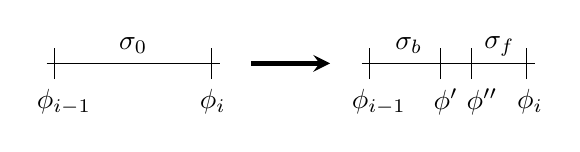
\begin{tikzpicture}
        \draw (-5.1, 0) -- (-2.9, 0);
        \draw (-5, -.2) -- (-5, .2);
        \draw (-3, -.2) -- (-3, .2);
        \node [below] at (-4.88, -.2) {$\phi_{i-1}$};
        \node [below] at (-2.99, -.2) {$\phi_i$};
        \node [above] at (-4, 0) {$\sigma_0$};

        \draw [ultra thick,->,>=stealth] (-2.5, 0) -- (-1.5, 0);

        \draw (-1.1, 0) -- (1.1, 0);
        \draw (-1, -.2) -- (-1, .2);
        \draw (1, -.2) -- (1, .2);
        \draw (.3, -.2) -- (.3, .2);
        \draw (-.1, -.2) -- (-.1, .2);
        \node [below] at (-.88, -.2) {$\phi_{i-1}$};
        \node [below] at (1.04, -.2) {$\phi_i$};
        \node [below] at (.43, -.2) {$\phi''$};
        \node [below] at (-.03, -.2) {$\phi'$};
        \node [above] at (.65, -.04) {$\sigma_f$};
        \node [above] at (-.5, 0) {$\sigma_b$};
    \end{tikzpicture}
    \caption{Diagram of the addition of two linking number constraints}
    \label{fig:lnc_diagram}
\end{figure}

We then put an angular restriction on the two new linking number constraints. By subtracting off the excess angle \(\phi\) that the undisturbed DNA has prior to RNAP binding we can define:
\begin{equation}
    \Delta \phi' = \phi' - \left(\phi_{i - 1} + \frac{z' - z_{i-1}}{z_i - z_{i-1}} (\phi_i - \phi_{i-1})\right)
\end{equation}

\begin{equation}
    \Delta \phi'' = \phi'' - \left(\phi_{i - 1} + \frac{z'' - z_{i-1}}{z_i - z_{i-1}} (\phi_i - \phi_{i-1})\right)
\end{equation}

For unwinding of the region bound to the RNAP to occur, we impose two constraints that ensure that the 13 base pairs that interact with the RNAP are fully unwound:
\begin{equation}
    |\Delta \phi'| + |\Delta \phi''| = 1.2 \cdot 2 \pi
\end{equation}
\begin{equation}
    \Delta \phi' - \Delta \phi'' = 1.2 \cdot 2\pi \label{eq:dphi_relation}
\end{equation}
For the intermediate region, this implies that there are two different ways to unwind the DNA; either to rotate the leading linking number constraint backwards or rotate the trailing linking number constraint forwards. There are also many intermediate solutions where \emph{both} of the bounding linking number constraints move. The first restriction is there to ensure that we use the solution that minimizes total amount of rotation needed.

Given a complete energy model that related \(\tau\) over the complete range of unwinding \(\Delta \phi', \Delta \phi''\) values, we could directly write the binding energy as
\begin{equation}
    \Delta E = \overline \tau' \Delta \phi' + \overline \tau'' \Delta \phi''
    \label{eq:direct_torque_calc}
\end{equation}
and minimize the energy cost with respect to \(\Delta \phi'\) or \(\Delta \phi''\), giving a unique solution for any specific geometry. As Marko's statistical mechanical model is likely not valid in the limit of complete unwinding, we instead move forward with this model by estimating the energy cost in both the ``exterior'' region and within the ``interior'', 13-bp region.

\subsubsection{Energy estimation in the exterior region}
If we assume that the energy surface is locally linear (e.g. in the exterior region, there is a small change in supercoiling density), then we can relate the instantaneous torque to the change in energy:
\[ \tau = \frac{1}{\omega_0} \frac{\partial S(\sigma)}{\partial \sigma}\]
for \(S\), the energy per unit length. This means that:
\begin{equation}
    \Delta E = (z_2 - z_1) \tau \omega_0 \Delta \sigma = (z_2 - z_1) \frac{\partial S}{\partial \sigma} \Delta \sigma
\end{equation}
By expanding the definition of \(\Delta \sigma\) for an arbitrary region bounded by two linking number constraints, we can actually recover the normal energy-torque definition:
\begin{equation}
    \Delta E_\text{external} = (z_2 - z_1) \tau \omega_0 \frac{\Delta\phi_2 - \Delta\phi_1}{\omega_0 (z_2 - z_1)} = \tau (\Delta \phi_2 - \Delta\phi_1) \label{eq:external_de}
\end{equation}
Note that this implies that the energy cost of linking number constraint rotation is independent of the region width; under a locally linear assumption, the energy cost depends only on the local instantaneous torque and the rotation angle. When is this valid? The change in supercoiling density in the exterior region is relatively low, \(O(0.05)\) as long as the region of interest is at least \(250bp\) away from the nearest linking number constraint on one of its sides. For promoter regions analyzed here, space between gene bodies ensures that this assumption holds.

\subsubsection{Energy estimation in the interior region (local melting)}
We can generally write the energy it takes to unwind the DNA in the interior region as an integral over the linear free energy density, \(S\):
\[\Delta E_\text{internal} =  \int_{\sigma_0}^{\sigma_0 + \Delta \sigma_\text{RNAP}} \Delta z_\text{RNAP} \frac{\partial S}{\partial \sigma} d\sigma\]

Given the well-defined structure of the RNAP-DNA complex and the fact that under all realistic physiological conditions \(\Delta \sigma_\text{RNAP} \gg \sigma_0\), we assume that the end-state energy is a constant, but unknown \(S_\text{unwound}\):
\begin{equation}
    \Delta E_\text{internal} = \Delta z_\text{RNAP} \left(S_\text{unwound} - S(\sigma_0)\right)
\end{equation}
While \(S_\text{unwound}\) is unknown, it is a constant with respect to all promoters, so this energetic term is implicitly already included in any promoter base rate. This means that the external energy depends only on the free energy density, evaluated at the local, initial supercoiling density \(\sigma_0\):
\begin{equation}
    \Delta E_\text{internal} = -\Delta z_\text{RNAP} S(\sigma_0) \label{eq:internal_de}
\end{equation}

\subsubsection{Order of magnitude energy analysis}
Combining the results of \cref{eq:external_de,eq:internal_de} and plugging in \cref{eq:dphi_relation}, we have an estimated binding energy:
\begin{equation}
    \Delta E = \tau(\sigma_0) 1.2 \cdot 2\pi - \Delta z_\text{RNAP} S(\sigma_0)
\end{equation}

When we plot this energetic term in \cref{fig:supp:energy_with_melting}, we see that the internal energetic term is minimal when compared to the external energetic term (local melting) at the supercoiling densities considered here, so we use the simplified form

\begin{equation}
    \Delta E = \tau(\sigma_0) \cdot 1.2 \cdot 2\pi
\end{equation}
as presented in \cref{eq:first_order_sc_initation}.

\end{document}
